\subsection{La geometría de las ecuaciones lineales}
\label{sec:1_la_geometria_de_las_ecuaciones_lineales}
\setcounter{equation}{0}
\setcounter{definition}{0}

Considere el siguiente sistema de ecuaciones lineales:\begin{align}
    \begin{cases}
        2x - y &= 1 \\
        x + y &=5
    \end{cases}
    \label{eq:1.1.1}
\end{align}

Este sistema de ecuaciones luce de la siguiente manera:

\begin{figure}[H]
    \centering
    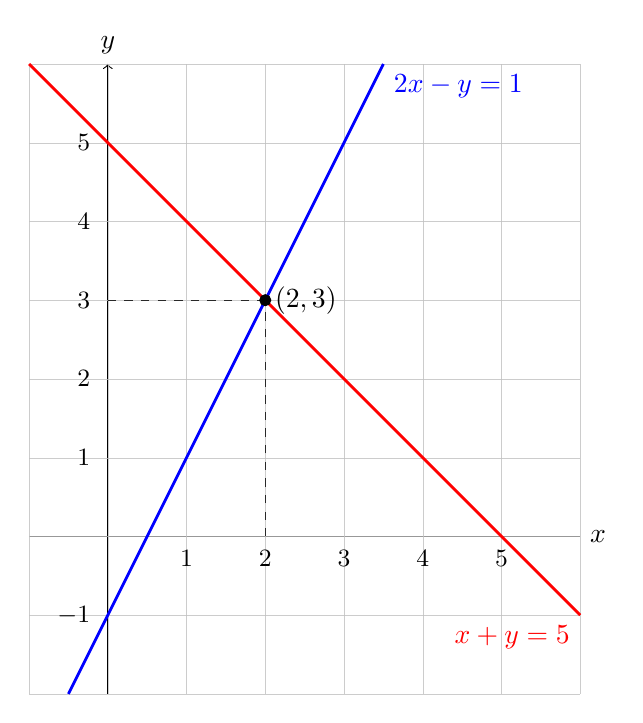
\begin{tikzpicture}
        % Axes:
        \draw[line width=0.4, color=black, arrows=->] (-1, 0) -- (6, 0)
                                                      (0, -2) -- (0, 6);
        
        % Labels:
        \node[anchor=west] at (6, 0) {$x$};
        \node[anchor=south] at (0, 6) {$y$};

        % Grid:
        \foreach \x in {-1, 0, 1, 2, 3, 4, 5, 6}
            \draw[line width=0.1, color=gray!50, opacity=0.8] (\x, -2) -- (\x, 6);
        \foreach \y in {-2, -1, 0, 1, 2, 3, 4, 5, 6}
            \draw[line width=0.1, color=gray!50, opacity=0.8] (-1, \y) -- (6, \y);
        
        % Labels in axes:
        \foreach \x in {1, 2, 3, 4, 5}
            \node[anchor=south] at (\x, -0.5) {\small{$\x$}};
        \foreach \y in {-1, 1, 2, 3, 4, 5}
            \node[anchor=east] at (-0.1, \y) {\small{$\y$}};

        % Functions:
        \draw[line width=1, color=blue] plot[domain=-0.5:3.5] (\x, 2*\x - 1) node[anchor=north west] {$2x - y = 1$};
        \draw[line width=1, color=red] plot[domain=-1:6] (\x, 5 - \x) node[anchor=north east] {$x + y = 5$};

        % Intersection dot at (2,3):
        \draw[line width=0.5mm, color=black, fill=black] (2, 3) circle (0.05);

        % Intersection dot label:
        \node[anchor=west] at (2, 3) {$\left(2, 3\right)$};

        % Intersection grid:
        \draw[line width=0.1, color=black, opacity=0.8, dashed] (0, 3) -- (2, 3);
        \draw[line width=0.1, color=black, opacity=0.8, dashed] (2, 0) -- (2, 3);
    \end{tikzpicture}
    \caption{Gráfica del sistema de ecuaciones lineales (\ref{eq:1.1.1}).}
    \label{fig:1.1.1}
\end{figure}

Ahora bien, existe una equivalencia entre representar un sistema de ecuaciones lineales en forma de gráfica y representarlo en forma de vectores. Para ello, considere el sistema de ecuaciones (\ref{eq:1.1.1}). Puede ser representado como: \begin{align}
    \underbrace{\begin{bmatrix}2 \\ 1\end{bmatrix}}_{\vec{v_1}} x + \underbrace{\begin{bmatrix}-1 \\ 1\end{bmatrix}}_{\vec{v_2}} y &= \underbrace{\begin{bmatrix}1 \\ 5\end{bmatrix}}_{\vec{b}}, \quad x,y \in \mathbb{R}
    \label{eq:1.1.2}
\end{align}

Dónde la gráfica de cada vector es la siguiente:

\begin{figure}[H]
    \centering
    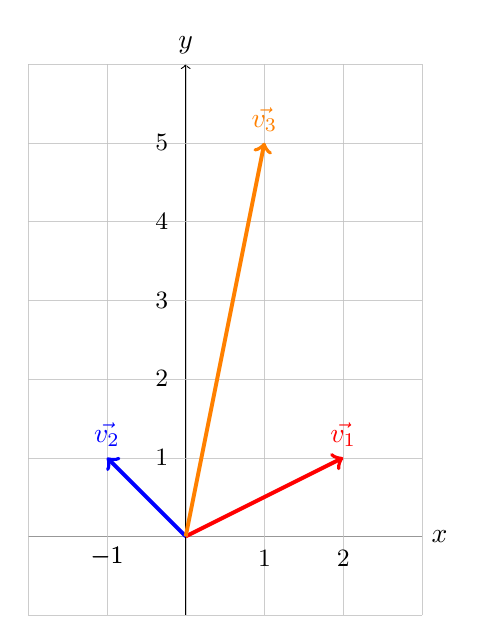
\begin{tikzpicture}
        % Axes:
        \draw[line width=0.4, color=black, arrows=->] (-2, 0) -- (3, 0)
                                                      (0, -1) -- (0, 6);
        
        % Labels:
        \node[anchor=west] at (3, 0) {$x$};
        \node[anchor=south] at (0, 6) {$y$};

        % Grid:
        \foreach \x in {-2, -1, 0, 1, 2, 3}
            \draw[line width=0.1, color=gray!50, opacity=0.8] (\x, -1) -- (\x, 6);
        \foreach \y in {-1, 0, 1, 2, 3, 4, 5, 6}
            \draw[line width=0.1, color=gray!50, opacity=0.8] (-2, \y) -- (3, \y);
        
        % Labels in axes:
        \foreach \x in {-1, -1, 1, 2}
            \node[anchor=south] at (\x, -0.5) {\small{$\x$}};
        \foreach \y in {1, 2, 3, 4, 5}
            \node[anchor=east] at (-0.1, \y) {\small{$\y$}};

        % Dependient vectors
        % \draw[line width=0.5mm, color=gray!80, dashed, opacity=0.5] (0, 0) -- (-3, 3);
        % \draw[line width=0.5mm, color=gray!80, dashed, opacity=0.5] (0, 0) -- (3, 1.5);
        
        % Vectors
        \draw[line width=0.5mm, color=red, arrows=->] (0, 0) -- (2, 1) node[anchor=south] {$\vec{v_1}$};
        \draw[line width=0.5mm, color=blue, arrows=->] (0, 0) -- (-1, 1) node[anchor=south] {$\vec{v_2}$};
        \draw[line width=0.5mm, color=orange, arrows=->] (0, 0) -- (1, 5) node[anchor=south] {$\vec{v_3}$};
    \end{tikzpicture}
    \caption{Óptica vectorial del sistema de ecuaciones (\ref{eq:1.1.1}).}
    \label{fig:1.1.2}
\end{figure}

\subsubsection{Álgebra de vectores}

\begin{enumerate}
    \item \textbf{Producto vectorial:} \begin{align*}
        v_1 \times v_2 = v_1 \times v_2^T &= \underbrace{\begin{pmatrix} \hspace*{0.1cm}\cdot\hspace*{0.1cm} \\ \hspace*{0.1cm}\cdot\hspace*{0.1cm} \end{pmatrix}}_{n\times1} \times \underbrace{\begin{pmatrix} \hspace*{0.1cm}\cdot\hspace*{0.1cm} & \hspace*{0.1cm}\cdot\hspace*{0.1cm} \end{pmatrix}}_{1\times n} = \underbrace{\begin{pmatrix} \hspace*{0.1cm}\cdot\hspace*{0.1cm} & \hspace*{0.1cm}\cdot\hspace*{0.1cm} \\ \hspace*{0.1cm}\cdot\hspace*{0.1cm} & \hspace*{0.1cm}\cdot\hspace*{0.1cm} \end{pmatrix}}_{\text{Matriz } n\times n}
    \end{align*}
    \item \textbf{Producto punto:} \begin{align*}
        v_1 \cdot v_2 &= v_1^T \cdot v_2 = \underbrace{\begin{pmatrix} \hspace*{0.1cm}\cdot\hspace*{0.1cm} & \hspace*{0.1cm}\cdot\hspace*{0.1cm} \end{pmatrix}}_{1\times n} \cdot \underbrace{\begin{pmatrix} \hspace*{0.1cm}\cdot\hspace*{0.1cm} \\ \hspace*{0.1cm}\cdot\hspace*{0.1cm} \end{pmatrix}}_{n\times1} = \underbrace{a}_{\mathbb{R}}
    \end{align*}
    \item \textbf{Producto por un escalar:} \begin{align*}
        \alpha v &= \alpha \begin{pmatrix} v_{11} \\ v_{21} \\ \vdots \\ v_{n1} \end{pmatrix} = \begin{pmatrix} \alpha v_{11} \\ \alpha v_{21} \\ \vdots \\ \alpha v_{n1} \end{pmatrix}
    \end{align*}
\end{enumerate}


\subsubsection{Variable compleja}
\label{sec:variable_compleja}

Sea $z$ una variable compleja, la cual está definida como: \begin{align}
    z = a + ib,
    \label{eq:1.1.3}
\end{align}

dónde, $a$ y $b$ son números reales y $i^2 = -1$.

\paragraph*{Operaciones con números complejos:}

\begin{enumerate}
    \item Suma: \begin{align*}
        z_1 + z_2 &= a_1 + ib_1 + a_2 + ib_2 \\
                    &= (a_1 + a_2) + (ib_1 + ib_2) \\
                    &= (a_1 + a_2) + i(b_1 + b_2)
    \end{align*}
    \item Multiplicación: \begin{align*}
        z_1 z_2 &= (a_1 + ib_1)(a_2 + ib_2) \\
                &= (a_1a_2 - b_1b_2) + i(a_1b_2 + a_2b_1)
    \end{align*}
\end{enumerate}

\subsection{Vectores y matrices}
\label{sec:vectores_y_matrices}

\begin{definition}[Vector renglón]
{
    \label{def:1.1.1}
    Sea $x$ un vector de $n$ dimensiones, entonces:
    \begin{align*}
        x = (x_1, x_2, \dots, x_n) \in \M_{(1 \times n)}
    \end{align*}
}
\end{definition}

\begin{definition}[Vector columna]
{
    \label{def:1.1.2}
    Sea $x$ un vector de $n$ dimensiones, entonces:
    \begin{align*}
        x = \begin{pmatrix}
            x_1 \\
            x_2 \\
            \vdots \\
            x_n
        \end{pmatrix} \in \M_{(n \times 1)}
    \end{align*}
}
\end{definition}

\begin{definition}[Matriz]
{
    \label{def:1.1.3}
    Sea $A$ una matriz de $m$ renglones y $n$ columnas, está definida como:
    \begin{align*}
        A = \begin{bmatrix}
            a_{11} & a_{12} & \cdots & a_{1n} \\
            a_{21} & a_{22} & \cdots & a_{2n} \\
            \vdots & \vdots & \ddots  & \vdots \\
            a_{m1} & a_{m2} & \cdots & a_{mn}
        \end{bmatrix} \in \M_{(m \times n)}
    \end{align*}
}
\end{definition}

\begin{definition}[Igualdad]
{
    \label{def:1.1.4}
    Sean $A$ y $B$ dos matrices de $m \times n$:
    \begin{align*}
        A = B \quad \Longleftrightarrow \quad \left[a_{ij}\right] = \left[b_{ij}\right], \quad \forall i \forall j
    \end{align*}
}
\end{definition}

\begin{definition}[Suma matricial]
{
    \label{def:1.1.5}
    Sean $A$, $B$ y $C$ matrices de $m \times n$:
    \begin{align*}
        A + B = C \Longleftrightarrow \left[ a_{ij} + b_{ij} \right] = \left[ c_{ij} \right]
    \end{align*}
}
\end{definition}

\begin{definition}[Multiplicación por un escalar]
{
    \label{def:1.1.6}
    Sean $A \in \M_{(m \times n)}$ y $\alpha \in \R$:
    \begin{align*}
        \alpha A = B, \quad B \in \M_{(m \times n)} \quad \Longleftrightarrow \quad \left[ \alpha a_{ij} \right] = \left[ b_{ij} \right]
    \end{align*}
}
\end{definition}

\begin{teorema}
{
    \label{thm:1}
    Sean $A$, $B$ y $C$ matrices de $m \times n$ y $\alpha, \beta$ números reales, entonces: \\

    \begin{enumerate}
        \item $A + \vec{0} = A$
        \item $0A = \vec{0}$
        \item $A + B = B + A$
        \item $(A + B) + C = A + ( B + C )$
        \item $\alpha ( A + B ) = \alpha A + \alpha B$
        \item $1A = A$
        \item $(\alpha + \beta) A = \alpha A + \beta A $
    \end{enumerate}
}
\end{teorema}

\subsection{Producto vectorial y producto matricial}
\label{sec:producto_vectorial_y_producto_matricial}

\begin{align*}
    \text{Sean } a = \begin{pmatrix}
        a_1 \\
        a_2 \\
        \vdots \\
        a_n
    \end{pmatrix} \text{ y } b = \begin{pmatrix}
        b_1 \\
        b_2 \\
        \vdots \\
        b_n
    \end{pmatrix}
\end{align*}

\paragraph*{Producto escalar (producto punto):}

\begin{align*}
    a \cdot b &= a_1b_1 + a_2b_2 + \cdots + a_nb_n \\
    &= a^Tb \\
    &= \begin{pmatrix} \hspace*{0.1cm}\cdot\hspace*{0.1cm} & \hspace*{0.1cm}\cdot\hspace*{0.1cm} & \hspace*{0.1cm}\cdot\hspace*{0.1cm} \end{pmatrix} \times \begin{pmatrix} \hspace*{0.1cm}\cdot\hspace*{0.1cm} \\ \hspace*{0.1cm}\cdot\hspace*{0.1cm} \\ \hspace*{0.1cm}\cdot\hspace*{0.1cm} \end{pmatrix} = \alpha, \quad \alpha \text{ es un escalar}
\end{align*}

% \begin{definition}[Producto escalar (producto punto)]
% {
%     \label{def:1.2.1}
%     \begin{align*}
%         a \cdot b &= a_1b_1 + a_2b_2 + \cdots + a_nb_n \\
%         &= a^Tb \\
%         &= \begin{pmatrix} \hspace*{0.1cm}\cdot\hspace*{0.1cm} & \hspace*{0.1cm}\cdot\hspace*{0.1cm} & \hspace*{0.1cm}\cdot\hspace*{0.1cm} \end{pmatrix} \times \begin{pmatrix} \hspace*{0.1cm}\cdot\hspace*{0.1cm} \\ \hspace*{0.1cm}\cdot\hspace*{0.1cm} \\ \hspace*{0.1cm}\cdot\hspace*{0.1cm} \end{pmatrix} = \alpha, \quad \alpha \text{ es un escalar}
%     \end{align*}
% }
% \end{definition}

\begin{teorema}
{
    \label{thm:2}
    Sean $a$, $b$ y $c$ vectores de $n$ dimensiones, es decir, $a$, $b$ y $c \in \R^n$ y sean $\alpha$, $\beta \in \R$, entonces: \\
    \begin{enumerate}
        \item $a \cdot \vec{0} = 0$
        \item $a \cdot (b + c) = a \cdot b + a \cdot c$
        \item $\alpha a \cdot b = \alpha (a \cdot b)$
    \end{enumerate}
}
\end{teorema}

\paragraph*{Producto matricial:}

Sean $A \in \M_{(m \times n)}$ y $B \in \M_{(n \times p)}$ y $C \in \M_{(m \times p)}$:
\begin{align*}
    AB = C, \quad \Longleftrightarrow \quad &\left[ a_{ij} \right] \cdot \left[ b_{ij} \right] = \left[ c_{ij} \right] \\
    &C_{ij} = \left[ A_{i\cdot} \right] \cdot \left[ B_{\cdot j} \right]
\end{align*}

% \begin{definition}[Producto matricial]
% {
%     \label{def:1.2.2}
%     Sean $A \in \M_{(m \times n)}$ y $B \in \M_{(n \times p)}$ y $C \in \M_{(m \times p)}$:
%     \begin{align*}
%         AB = C, \quad \Longleftrightarrow \quad &\left[ a_{ij} \right] \cdot \left[ b_{ij} \right] = \left[ c_{ij} \right] \\
%         &C_{ij} = \left[ A_{i\cdot} \right] \cdot \left[ B_{\cdot j} \right]
%     \end{align*}
% }
% \end{definition}

\begin{teorema}
{
    \label{thm:3}
    Sean $A \in \M_{(n, m)}$, $B \in \M_{(m, p)}$ y $C \in \M_{(p, q)}$, entonces: \\
    \begin{align*}
        A(BC) = (AB)C
    \end{align*}
}
\end{teorema}

\begin{teorema}
{
    \label{thm:4}
    Sean $A \in \M_{(n, m)}$ y $B, C \in \M_{(m, p)}$, entonces: \\
    \begin{align*}
        A (B + C) = AB + AC
    \end{align*}
}
\end{teorema}

\begin{teorema}
{
    \label{thm:5}
    Sean $A, B \in \M_{(n, m)}$ y $C \in \M_{(m, p)}$, entonces: \\
    \begin{align*}
        (A + B)C = AC + BC
    \end{align*}
}
\end{teorema}

\subsection{Representación matricial de sistemas de ecuaciones lineales}
\label{sec:representacion_matricial_de_sistemas_de_ecuaciones_lineales}

Sean $A \in \M_{(n, n)}$ y $x, b \in \R^n$:

\begin{align*}
    Ax = b, \quad \longrightarrow \quad &\begin{cases}
        \text{\textbf{Sistema no homogéneo}} \\ 
        \text{Puede o no tener solución}
    \end{cases} \\
    Ax = \vec{0}, \quad \longrightarrow \quad &\begin{cases}
        \text{\textbf{Sistema homogéneo}} \begin{cases}
            x = \vec{0} \rightarrow \text{Solución trivial} \\
            \text{Múltiples soluciones}
        \end{cases}\\
        \text{Siempre tiene solución}
    \end{cases}
\end{align*}

\begin{teorema}
{
    \label{thm:6}
    Sean $x_1$ y $x_2$ soluciones del \textit{sistema no homogeneo}. Entonces su diferencia $x_1 - x_2$ es una solución del \textit{sistema homogéneo} asociado. \\

    \textbf{D!} Sean $x_1, x_2, b \in \R^n$ y $A \in \M_{(n, n)}$, entonces:
    \begin{align*}
        Ax_1 &= A(x_1 - x_2) \\
            &= Ax_1 - Ax_2 \\
            &= b - b \\
            &= \vec{0}
    \end{align*}\qed

    Otra demostración: \\

    \textbf{D!} Sean $x_1, x_2, b \in \R^n$ y $A \in \M_{(n, n)}$, entonces:

    \begin{align*}
        Ax_1 = b \quad & \quad Ax_2 = b \\ \\
        Ax_1 &= Ax_2 \\
        Ax_1 - Ax_2 &= \vec{0} \\
        A(x_1 - x_2) &= \vec{0} \\
        Ax &= \vec{0}
    \end{align*}\qed
}
\end{teorema}

\begin{corolario}
{
    Si $x$ es una solución del \textit{sistema no homogéneo}, $y$ es otra solución del \textit{sistema no homogéneo}, entonces, existe una solución $h$ al \textit{sistema homogéneo} asociado tal que:
    \begin{align*}
        y = x + h
    \end{align*}
    \textbf{D!} \begin{align*}
        h &= y - x \\
        h &= x \\
        Ax &= A(y - x) \\
        &= Ay - Ax \\
        &= b - b \\
        &= \vec{0}
    \end{align*}\qed \\

    \begin{note}
        [
            Si el fin es encontrar todas las soluciones del \textit{sistema no homogéneo}, entonces, se puede tomar $x$ como una solución cualquiera y $y$ como la solución del \textit{sistema homogéneo} asociado a $x$.
        ]
    \end{note}
}
\end{corolario}

\subsection{Matrices inversas}
\label{sec:matrices_inversas}

Si una matriz $A$ tiene inversa, entonces $A$ es \textbf{invertible} y $A^{-1}$ es la \textbf{matriz inversa} de $A$.

\begin{definition}[Matriz inversa]
{
    \label{def:1.2.3}
    Sean $A \in \M_{(n, n)}$ y $B \in \M_{(n, n)}$:
    \begin{align*}
        AB = BA = I_n
    \end{align*}
    dónde $B$ es la matriz inversa de $A$ y $I_n$ es la matriz identidad de orden $n$.
    \begin{align*}
        AA^{-1} = A^{-1}A = I_n
    \end{align*}
}    
\end{definition}

La pregunta es: ¿$A$ es invertible?

\begin{itemize}
    \item Si $\text{det}(A) \neq 0$, entonces $A$ es invertible.
    \item Si $\text{det}(A) = 0$, entonces $A$ no es invertible, es decir, no tiene inversa.
    \item $\left[ A | I_n \right] \Longrightarrow \left[ I_n | A^{-1} \right]$ \\ $A$ es invertible si es posible llegar a la matriz identidad en la parte izquierda de la matriz aumentada. \\ Si $A$ es una matriz cuadrada de $n \times n$, entonces debe obtener $n$ pivotes en la matriz aumentada. Algo como lo siguiente: \\ \begin{align*}
        \begin{bmatrix}
            1 & \xi & \xi & \xi & \cdots & \xi \\
            0 & 1 & \xi & \xi & \cdots & \xi \\
            0 & 0 & 1 & \xi & \cdots & \xi \\
            0 & 0 & 0 & 1 & \cdots & \xi \\
            \vdots & \vdots & \vdots & \vdots & \ddots & \vdots \\
            0 & 0 & 0 & 0 & \cdots & 1
        \end{bmatrix}
    \end{align*}
    Si hay menos de $n$ pivotes, entonces $A$ no es invertible.
\end{itemize}

\begin{note}
[
    La matriz inversa de la matriz inversa de una matriz $A$ es $A$:
    \begin{align*}
        (A^{-1})^{-1} = A
    \end{align*}
]
\end{note}

\begin{teorema}
{
    \label{thm:7}
    Si $A$ es invertible, entonces su matriz inversa $A^{-1}$ es única. \\

    \textbf{D!} Sean $A, B, C \in \M_{(n, n)}$, tales que $B$ y $C$ son matrices inversas de $A$. Entonces:
    \begin{align*}
        BA = AB = I_n \quad & \quad \quad CA = AC = I_n \\ \\
        B &= BI \\
        &= B(AC) \\
        &= BA(C) \\
        &= IC \\
        &= C \\ \\
        \therefore \quad B &= C \quad \text{\textbf{\large{!}}}
    \end{align*}\qed \\

    Esto es una contradicción, ya que $B$ y $C$ son matrices inversas de $A$, que al principio se habían supuesto distintas. Sin embargo, la demostración anterior muestra que son iguales.
}
\end{teorema}

\begin{teorema}
{
    \label{thm:8}
    Si $(AB)$ es invertible, entonces $B^{-1}A^{-1}$ es la matriz inversa de $(AB)$.
    \begin{align*}
        (AB)(AB)^{-1} &= (AB)^{-1}(AB) = I_n \\
        ABA^{-1}B^{-1} &= A^{-1}B^{-1}AB = I_n \\
    \end{align*}
}
\end{teorema}